\chapter{How does X Influence Novelty, Complexity, and Adaptation?}
\label{ch:influencing-cna}

\section{Event-driven vs. Sensor-driven Genetic Encoding}

SignalGP is a biologically-inspired approach that allows digital organisms to dynamically respond to environmental signals.
Each event (i.e., a signal from the environment or other agent) is associated with a tag to identify it; modules in the digital organism will be triggered to execute when an event with a matching tag occurs (Figure \ref{fig:signalgp-schematic;ch:influencing-cma}) \citep{lalejini2018evolving}.

We have shown that SignalGP allows evolved programs to engage in a broad range of environmental interactions and can better incorporate context into their behaviors.
Lalejini et. al. found that tag-based genetic regulation dramatically improved the solution success rate on sensor-intensive and context-dependent problems \citep{lalejini2018evolving, lalejini2021tag}.
Despite these positive results, this methodology has not yet been directly examined in an artificial life context, especially for its capacity to produce biologically realistic interactions.
Our goal is to enrich the toolbox of artificial life researchers to conduct evolution experiments while also expanding the applications to genetic programming.

\begin{figure}[h]

\centering
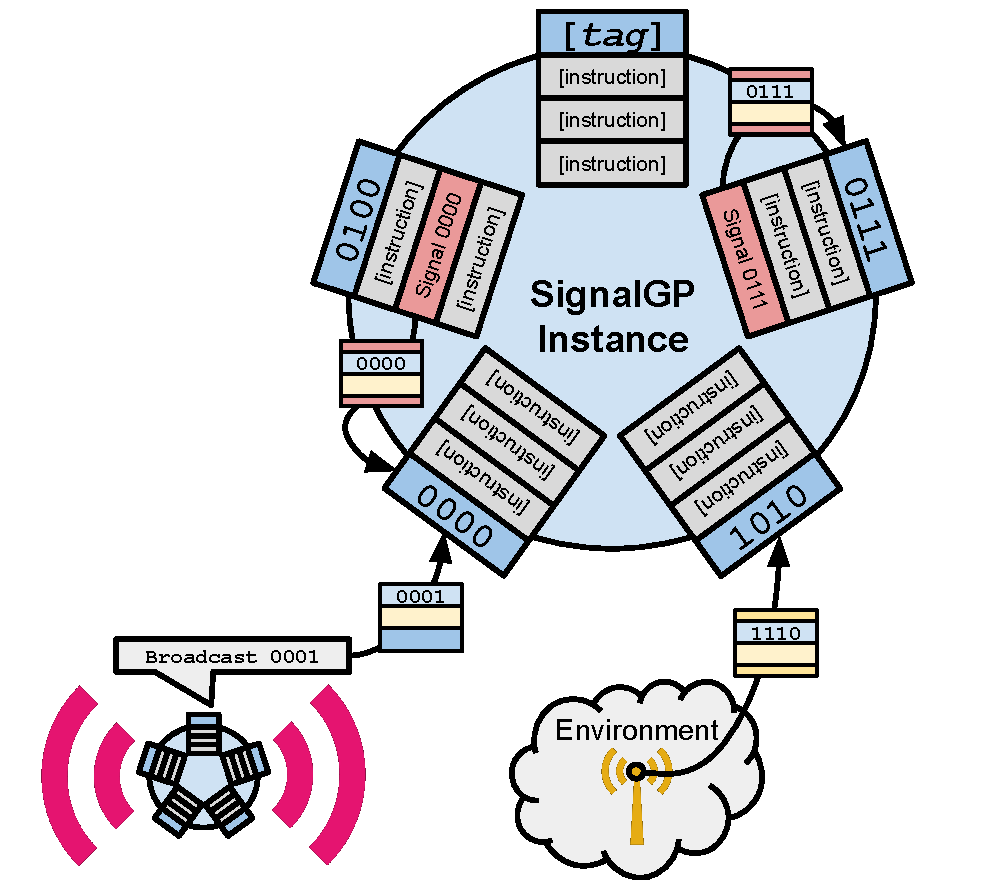
\includegraphics[width=0.5\textwidth]{img/signalgp-schematic}

\caption{SignalGP schematic depicting interactions between an agent and its environment}
\label{fig:signalgp-schematic;ch:influencing-cna}

\end{figure}


DISHTINY is a digital framework designed to study open-ended transitions to multicellularity \citep{moreno2019toward}.
In preliminary studies, we have used SignalGP in DISHTINY to enable dynamic interactions among cells and between cells and their environment, resulting in complex and diverse multi-cellular organisms.
Existing work with DISHTINY has focused on studying the evolution of multicellular traits, but not on characterizing the genetic programming methodology that underpins it.

Our experimental treatment will supplement procedural sensor instructions with corresponding event cues.
We will conduct control treatments where we modify signal function on multicellular organisms to isolate the impact of these event-driven cues.  Specifically we will (1) disable signals, (2) randomize signals, (3) temporally offset signals, and (4) spatially offset signals to disentangle their effects and importance.
We will assess the impact of event-driven cues in terms of:
\begin{itemize}
\item amount of environmental information agents incorporate into adaptive behaviors,
\item overall fitness of evolved behavioral strategies, and
\item behavior complexity, measured as number genome sites that contribute to fitness.
\end{itemize}

Establishing how SignalGP affects these metrics is critical to understanding how to effectively employ it, and will ultimately advance experimentally-driven studies of evolution in action.

\section{Alternate Proposals}

\begin{itemize}
  \item Role of sexual recombination (too broad)
  \item Role of ecology
  \item Selecting for multicell ``functionality''
  \begin{itemize}
    \item Idea: motility
    \begin{itemize}
      \item Increase resource collection rate based on distance from which kin group ID originated
    \end{itemize}
    \item Idea: distributed sensing
    \begin{itemize}
      \item Generate an underlying state (T/F) for each kin group id,
      \item Each cell can sense the underlying state, but with an unreliable sensor
      \item Increase resource collection rate based on consensus for the correct underlying state
      \item Could also try some sort of pattern sensing (vertical vs horizontal stripes, etc)
    \end{itemize}
    \item Idea: Resource exchange
    \begin{itemize}
      \item Generate and randomly distribute resource ``tokens''
      \item ``Tokens'' may be beneficial or harmful when ``cashed in,'' based on kin group ID (i.e., good for some groups harmful for others)
      \item Allow cells (and groups) to exchange tokens
      \item This could simulate “trading” between groups or “specialization” within groups
    \end{itemize}
  \end{itemize}
\end{itemize}
